\chapter{Lecture 2}
\section{Prefix Free Codes}
\begin{eg}
    Consider $\Ucal = \{a,b,c\}$ and consider two codes
    \begin{align*}
        c:&\quad c(a) = 0,\; c(b) = 10,\; c(c) = 11 \\
        \widetilde{c}:& \quad\widetilde{c}(a) = 0,\; \widetilde c(b) = 01, \; \widetilde c(c) = 11
    \end{align*}
    The first code is prefix free, and hence is uniquely decodable. The second is not prefix free, but we can still uniquely decode it! To do so, when we receive the entire sequence of bits, we reverse the sequence and apply decode it as if it was encoded using code $c$ (note that $\widetilde c$ is the reverse of $c$).
\end{eg}
A point to note is that in the second case, we might need to store an arbitrary length binary representation before we can decode the first letter and hence we require a Turing Machine! But in the first case, we need only a finite memory since we can decode the first letter when the required number of bits come in. For this reason, prefix free codes are also called \textbf{instantaneously decodable} codes. The above example also showed that although all prefix free codes are uniquely decodable, the reverse is not true. There exist uniquely decodable codes which are not prefix free.

\begin{figure}[h]
    \centering
    \begin{tikzpicture}[scale=0.7, framed, background rectangle/.style={thick, draw=black}]
\def\angle{60}%
\pgfmathsetlengthmacro{\xoff}{2cm*cos(\angle)}%
\pgfmathsetlengthmacro{\yoff}{1cm*sin(\angle)}%
\draw [thick, fill=gray!10] (\xoff,\yoff) circle[x radius=8cm, y radius=4cm] ++(3*\xoff,3*\yoff) node{Injective};
\draw [thick, fill=gray!50] (0.5*\xoff,0.5*\yoff) circle[x radius=5cm, y radius=2.5cm] ++(1.5*\xoff,1.5*\yoff) node{Uniquely Decodable};
\draw [thick, fill=gray!80] (0,0) circle[x radius=2cm, y radius=1cm] node{Prefix Free};
\end{tikzpicture}

    \caption{The box represents all codes possible, prefix free codes are a small category of it.}
\end{figure}
\begin{remark}
Although prefix free codes are a subset of uniquely decodable codes, there is no inherent advantage of using non prefix free codes which are uniquely decodable.
\end{remark}
\begin{theorem}
Suppose $c:\Ucal \to \binset$ for which $\ks(c) \leq 1$. Then $\exists$ a code $\widetilde{c}: \Ucal \to \binset$ s.t. 
\begin{itemize}
    \item $\widetilde{c}$ is prefix free
    \item $\ell_{\widetilde{c}}(u) = \ell_c(u) \;\forall \;u$
\end{itemize}
\end{theorem}
\begin{proof}
Let $\Ucal = \{1,2,\dots, k\}$ and let $\ell_1 = \ell_c(u_1), \dots \ell_k = \ell_c(u_k)$ s.t. $\ell_1 \leq \ell_2 \leq \cdots \leq \ell_k$. It is also known that $\sum_i 2^{-\ell_i} \leq 1$. \\
\begin{minipage}{0.65\textwidth}
Consider the complete binary tree on the right. It is constructed starting from $null$ and each time you grow each level one bit at a time. Each parent is a prefix of its children. Now we consider the following algorithm: 
\begin{enumerate}
    \item Start with the complete binary tree of depth $\ell_k$ as shown in the figure. In the beginning, mark every node as available
    \item For $i=1,\dots,k$:
    \begin{itemize}
        \item Find a node available at depth $\ell_i$ (say it is $n_i$)
        \item Set $\widetilde{c}(i) = n_i$
        \item Mark the node $n_i$ and all if its ascendants as unavailable
    \end{itemize}
\end{enumerate}
\end{minipage}
\hspace{0.1\textwidth}
\begin{minipage}{0.25\textwidth}
\begin{tikzpicture}[grow'=up, color=purple]
        \Tree [.$null$ [.0 [.00 [.. ] [.. ] ] [.01 [.. ] [.. ] ] ]
                   [.1 [.10 [.. ] [.. ] ] [.11 [.. ] [.. ] ] ] ]
\end{tikzpicture}
\end{minipage}
Although the algorithm does find such a $\widetilde{c}$, we need to rigorously show that we can always find a node at depth $\ell_i$. To show this, notice that at the beginning of the algorithm, there were $2^{\ell_i}$ nodes at depth $\ell_i$. At every iteration until $i-1$, some nodes at depth $\ell_i$ get marked unavailable. Hence, at the $i^{th}$ iteration, we have the number of available nodes as
\[\text{\# available nodes} = 2^{\ell_i} - \sum_{j=1}^{i-1} 2^{\ell_i - \ell_j} = 2^{\ell_i}\bigg[1-\sum_{j=1}^{i-1} 2^{-\ell_j}\bigg]\]
Since the Kraft Sum is at most 1, we have $\sum_{j=1}^{i-1} 2^{-\ell_j} < 1$ strictly. Hence the RHS of the above equation is always positive. But since it is just a difference of integers, the RHS must be at least 1. Hence, the algorithm executes successfully and we can construct such a $\widetilde{c}$.
\end{proof}
\section{The Logarithm}
\begin{lemma}
$\ln(z) \leq z-1$ and equality only occurs at $z=1$
\end{lemma}
\begin{proof}
We consider the finite Taylor's expansion of $\ln(z)$ around $z=1$. \\
\begin{minipage}{0.6\textwidth}
Recall that, the Taylor series expansion of $f(z)$ around $z_0$, for $\alpha$ between $z$ and $z_0$ is given as
\[f(z) = f(z_0) + (z-z_0)f'(z_0) + \frac{1}{2}(z-z_0)^2 f''(\alpha) \]
\begin{align*}
   \implies \ln(z) &= \ln(1) + (z-1) \cdot 1 + \frac{1}{2} (z-1)^2 \cdot \bigg(-\frac{1}{2\alpha^2}\bigg) \\
    &= (z-1) - \frac{1}{2}\bigg(\frac{z-1}{\alpha}\bigg)^2 \leq z-1
\end{align*}

\end{minipage}
\hspace{0.1\textwidth}
\begin{minipage}{0.3\textwidth}
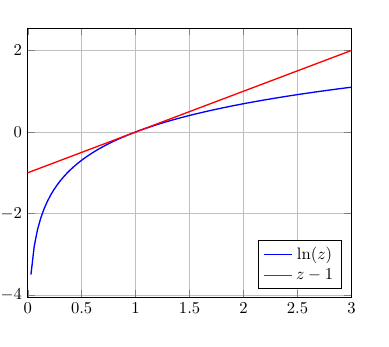
\begin{tikzpicture}[trim axis left, scale=0.6]
\begin{axis}[domain=0:3,
  samples=100,
  enlarge x limits=false,
  grid=both,
  no markers,
  legend pos=south east]
\addplot +[thick] {ln(x)};
\addlegendentry{$\ln(z)$};
\addplot +[thick] {x-1};
\addlegendentry{$z-1$};
\end{axis}
\end{tikzpicture}
\end{minipage}
\end{proof}
\begin{corollary}
Suppose $p_1, \dots, p_k \geq 0$ are such that $\sum_i p_i = 1$. Suppose $z_1, \dots, z_k > 0$, then we have
\[\sum_i^k p_i \ln(z_i) \leq \ln\bigg(\sum_{i=1}^k p_iz_i\bigg)\]
with equality only when $z_1 = z_2 = \cdots = z_k$.
\end{corollary}
\begin{proof}
Let $\mu = \sum_i p_i z_i$ and we need to show that 
\begin{align*}
&\sum_i p_i \ln(z_i) \leq \ln \mu \implies \sum_i p_i \bigg[\ln\Big(\frac{z_i}{\mu}\Big)\bigg] \leq 0
\end{align*}
Using the previous lemma, we have
\[\sum_i p_i \bigg[\ln\Big(\frac{z_i}\mu\Big)\bigg] \leq \sum_i p_i \bigg[\frac{z_i}{\mu} - 1\bigg] = \frac{1}{\mu} \sum_i{p_iz_i} - \sum p_i = 0\]
\end{proof}
\begin{definition}
Suppose $p$ is a probability distribution on $\Ucal$ and suppose $q:\Ucal \to [0,\infty)$. Then we define the Kullbeck-Liebler Divergence as
\[\kl pq \triangleq \sum_u p(u) \log\Big(\frac{p(u)}{q(u)}\Big)\]
\end{definition}
\begin{remark}
If for any $u$, $p(u) = 0$, we consider the value of the term to be $0$, and if for any $u$, $q(u) = 0$, then we say that $\kl pq \to \infty$.
\end{remark}
\begin{lemma}
$\kl pq \geq - \log\big(\sum_u q(u)\big)$
\end{lemma}
\begin{proof}
\begin{align*}
    -\kl pq &= \sum_u p(u) \log\Big(\frac{p(u)}{q(u)}\Big) \\
    &\leq \log\bigg[\sum_u p(u) \frac{q(u)}{p(u)}\bigg] = \log\big(\sum_u q(u)\big) \\
\implies \kl pq &\geq -\log\big(\sum_u q(u)\big)
\end{align*}
\end{proof}
\begin{remark}
In particular when $q$ is also a probability distribution on $\Ucal$, we have $\kl pq \geq 0$.
\end{remark}
Suppose we have an alphabet $\Ucal$, a distribution $p$ defined on $\Ucal$ and a code $c: \Ucal \to \binset$. If we choose a letter $U$ randomly from the alphabet using the probability distribution, we can say that $\EE[\ell(U)]$ denotes the expected number of bits representing a letter.
\begin{eg}
Consider $\Ucal = \{a,b,c,d,e\}$, let $p = (0.3, 0.1, 0.15, 0.2, 0.25)$ and $c = (00, 01, 10, 110, 111)$. Then we have
$\EE[\ell(u)] = 0.3\times 2 + 0.1\times 2 + 0.15\times2+0.2\times3 + 0.15\times 3 = 2.45$
\end{eg}
\begin{theorem}
For any code $c: \Ucal \to \binset$ and a probability distribution $p$ defined on $\Ucal$, we have
\[\EE[\ell(u)] \geq \sum_u p(u) \log_2 \frac{1}{p(u)} - \log_2 [\ks(c)]\]
In particular, when $c$ is uniquely decodable, we have
\[\EE[\ell(u)] \geq \sum_u p(u) \log_2 \frac{1}{p(u)}\]
\end{theorem}
\begin{proof}
We define $q$ on $\Ucal$ as $q(u) = 2^{-\ell(u)} \implies \ell(u) = \log_2 \frac{1}{q(u)}$. Noticing the correspondence, we can write $\EE[\ell(u)] = \sum_u p(u) \log_2\frac{1}{q(u)} = \kl pq + \sum_u p(u)\log\frac{1}{p(u)}$. Now, we have 
\begin{align*}
    \EE[\ell(u)] &= \sum_u p(u) \log\frac{1}{p(u)} + \kl pq \\
    &\geq \sum_u p(u) \log\frac{1}{p(u)} - \log(\sum q(u)) \\
    &= \sum_u p(u) \log\frac{1}{p(u)} - \log \ks(c)
\end{align*}
\end{proof}
\begin{theorem}
Given $\Ucal, p$, $\exists$ a prefix free code $c$ s.t.
\[\EE[\ell(u)] \leq \sum p(u) \log \frac{1}{p(u)} + 1\]
\end{theorem}
\begin{proof}
We set $\ell(u) \triangleq \lceil \log_2 \frac{1}{p(u)} \rceil$. Due to the ceil function, it is clear that $\sum_u 2^{-\ell(u)} \leq 1$ (it was an equality without the ceil). 
We have
\begin{align*}
    \ell(u) &\leq \log_2 \frac{1}{p(u)} + 1 \\
    \implies \EE[\ell(u)] &\leq \sum_u p(u) \log\frac{1}{p(u)} + 1
\end{align*}
\end{proof}